%% AMS-LaTeX Created with the Wolfram Language for Students - Personal Use Only : www.wolfram.com

\documentclass{article}
\usepackage{amsmath, amssymb, graphics, setspace}

\newcommand{\mathsym}[1]{{}}
\newcommand{\unicode}[1]{{}}

\begin{document}

\text{Clear}[\text{Global$\grave{ }$*}]\\
\text{eigenstates}[\gamma \_,\epsilon \_,\text{ndiv$\_$},\text{l$\_$}]\text{:=}\\
\text{Module}[\{\text{dx},\text{npts},\text{mat},\text{bvec},\text{phi}\},\\
\text{dx}=N[l/\text{ndiv}];\\
\text{npts} = \text{ndiv}-1;\\
\text{mat} = \text{Table}[\text{If}[i\text{==}j,(-2/\text{dx}{}^{\wedge}2)-(\gamma  j \text{dx}),0]+\text{If}[\text{Abs}[i-j]\text{==}1,1/\text{dx}{}^{\wedge}2,0],\{i,1,\text{npts}\},\{j,1,\text{npts}\}];\\
\text{bvec} = \text{Table}[-\epsilon ,\{j,1,\text{npts}\}];\\
\text{bvec}[[1]]=0;\\
\text{bvec}[[\text{npts}]]=0;\\
\text{phi} = \text{LinearSolve}[\text{mat}, \text{bvec}];\\
\text{phiTot} = \text{Join}[\{0\},\text{phi},\{0\}];\\
\text{phidat} = \text{Table}[\{(j-1)*\text{dx},\text{phiTot}[[j]]\},\{j,1,\text{ndiv}+1\}]\\
];\\
\gamma _{\text{large}}=10{}^{\wedge}3;\\
\gamma _{\text{small}}=10{}^{\wedge}(-3);\\
\epsilon =1;\\
l=1;\\
\text{ndiv}=100;\\
\text{small} = \text{eigenstates}\left[\gamma _{\text{small}},\epsilon ,\text{ndiv},l\right];\\
\text{large} = \text{eigenstates}\left[\gamma _{\text{large}},\epsilon ,\text{ndiv},l\right];\\
\text{ListPlot}[\text{small},\text{Joined}\to \text{True},\text{PlotLabel}\to \text{Small value of $\gamma $}]\\
\text{ListPlot}[\text{TakeSmallest}[\text{small}[[\text{All}, 2]],10],\text{Joined}\to \text{True},\text{PlotLabel}\to \text{Smallest Values: Small
value of $\gamma $}]\\
\text{ListPlot}[\text{large},\text{Joined}\to \text{True},\text{PlotLabel}\to \text{Large value of $\gamma $}]\\
\text{ListPlot}[\text{TakeSmallest}[\text{large}[[\text{All}, 2]],10],\text{Joined}\to \text{True},\text{PlotLabel}\to \text{Smallest Values: Large
value of $\gamma $}]\\
\text{lowestEigenstates} = \text{Table}[\text{TakeSmallest}[\text{Select}[\text{eigenstates}[10*j,\epsilon ,\text{ndiv},l][[\text{All},2]],\#>0\&],2],\{j,0,100\}];\\
\text{ListPlot}[\text{Transpose}[\text{lowestEigenstates}],\text{Joined}\to \text{False},\text{PlotLabel}\to \text{Lowest eigenstates}]

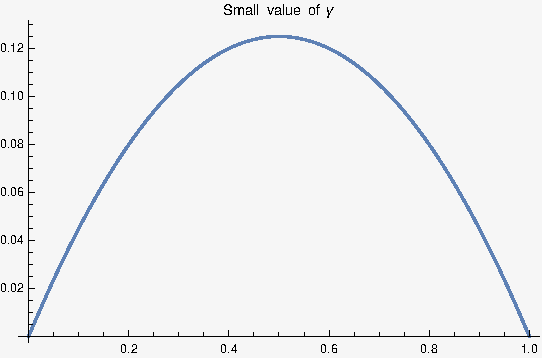
\includegraphics{q_6_gr1.eps}

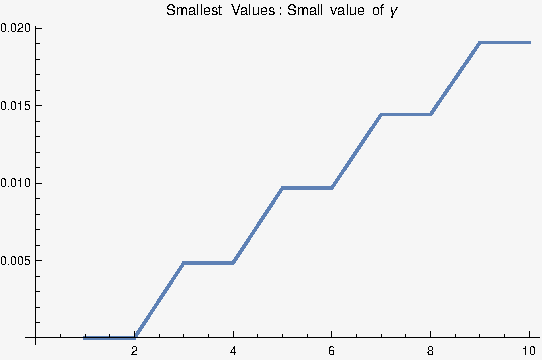
\includegraphics{q_6_gr2.eps}

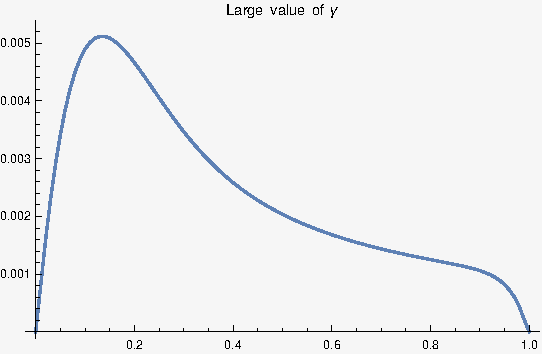
\includegraphics{q_6_gr3.eps}

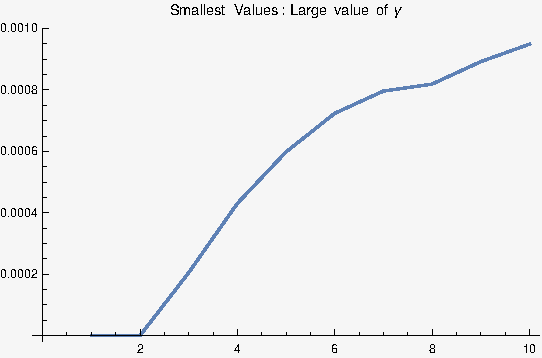
\includegraphics{q_6_gr4.eps}

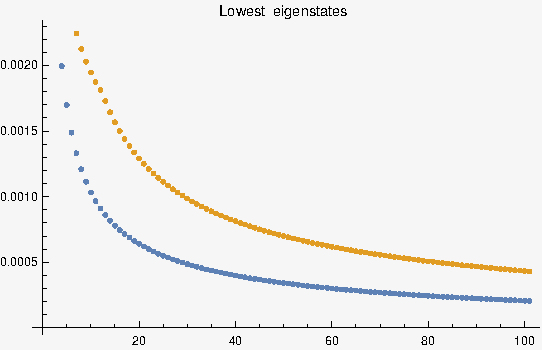
\includegraphics{q_6_gr5.eps}

|

\end{document}
